\newpage
\section{Problema 2: Problemas en el camino}

\subsection{Introducción}
	El siguiente obstáculo del grupo de arqueólogos consiste en reconstruir el estado de una balanza de dos platillos con una carga $P$ del lado izquierdo utilizando únicamente pesas de distintas potencias de 3. Además la solución propuesta debe tener complejidad temporal del orden $\mathcal{O}(\sqrt(P))$
	\\

	Por la naturaleza del problema, donde nos interesa determinar únicamente la pertenencia de cada potencia en el total de las que usamos para nivelar la balanza (y distinguir a qué lado de la balanza van) la representación del estado final de cada platillo por separado mediante conjuntos disjuntos resulta apropiada. Llamaremos $I$ al conjunto final de las potencias sobre el platillo izquierdo y $D$ a aquellas de la derecha. Además, como cada plato es contrapeso del otro, el estado de la balanza respecto de uno de los platillos se interpreta como su carga menos la del opuesto.
	\\

	A partir de dichas representaciones, dado un valor de $P$, queremos encontrar dos conjuntos disjuntos de potencias de base 3 $I$ y $D$ tales que recreen el estado de la balanza original con una única carga $P$ a la izquierda. Formalmente:

$$
    I,D \subset \{3^n \;|\; n \in \mathbb{N}_0 \} \;\; \land \;\;
    \sum I - \sum D = P \;\; \land \;\;
    I \cap D = \emptyset
$$

	Por ejemplo, para $P$ = 34 el par de conjuntos $\left \langle I,D  \right \rangle$ = $\left \langle \{27,9,1\},\{3\}  \right \rangle$ es solución porque \\
	$\{27,9,1\} \cap \{3\} = \emptyset \ \wedge \ 34 = \sum I - \sum D = (27+9+1)-(3)$.
	\\



\subsection{Solución y Correctitud}
	Para poder determinar $I$ y $D$ utilizaremos la descomposición polinómica base 3 de $P$. El caso más simple de analizar es cuando $P$ es una potencia de 3 y entonces solamente requerimos de un único elemento para $I$ (es decir, el mismo $P$) y ninguno para $D$. En realidad este es un subcaso de otro más general: que la representación en base 3 de $P$ sea binaria (no haya dígitos que valen 2). Estos casos se pueden resolver fácilmente con $I$ como el conjunto de todos los monomios de la descomposición polinómica, es decir, los dígitos de su representación ternaria. Formalizando, sea $P_{10}$ = $A_3$ = $\left \langle a_{ \left \lfloor{log(P)}\right \rfloor + 1 } \ ... \ a_1, a_0  \right \rangle$ por definición entonces \\

	$P$ = $\sum_{i = 0}^{\left \lfloor{log(P)}\right \rfloor + 1} a_i*3^{i}$ y nos alcanza con tomar $I$ = $\bigl ( \ \bigcup_{i=0}^{\left \lfloor{log(P)}\right \rfloor + 1} \{a_i*3^{i}\} \ \bigr ) \setminus \{0\} \ \ y \ \ D = \emptyset $
	\\

	Sin embargo, hasta ahora obviamos qué sucede si hay coeficientes que valen 2 en la descomposición polinómica de $P$. Retornando a modo ilustrativo al contexto narrativo del problema, no poseemos múltiples pesas de un mismo peso. Es decir que, manteniendo por base la idea para el caso anterior, necesitamos alguna mecánica que garantice la existencia de una solución a costa de cargar valores en $D$ que complementen manipulaciones en $A_3$ para determinar $I$.
	\\

	La algoritmia de la solución trata en recorrer, desde el menos significativo, cada uno de los dígitos $a_i$ de $A_3$, la representación ternaria de $P$, y determinar para ambos conjuntos si $3^{i}$ pertenece a alguno. Como la base está implícita, únicamente guardamos los índices o exponentes $i$ a medida que los recorremos, quedando ordenados crecientemente, y nos encargamos luego de reproducir los verdaderos elementos de $I$ y $D$ elevando 3 a cada exponente. Entonces usamos secuencias $der$ e $izq$ que cumplen:
	\\

	$D = \bigcup_{j=0}^{|der|-1} \{3^{der_{j}}\}  $   \quad (ídem para $izq$ con $I$)
	\\

	Manteniendo la idea del primer caso, cuando el dígito $a_i$ sea 1 entonces agregamos el exponente $i$ al conjunto $I$, de ser 0 seguimos recorriendo. De este modo seguimos tomando a $A_3$ como base para $I$ aprovechando que tomar los términos de la descomposición polinómica de $P$ para $I$ y $D = \emptyset$ siempre cumple la condición $\sum I$ - $\sum D$ = $P$. Nos queda ver cómo deshacernos de los términos con coeficientes iguales a 2.

	Pero si $a_i$ es 2 lo que hacemos es contar ese exponente para $D$ y provocamos un acarreo hacia el próximo dígito $a_{i+1}$ que pasa a valer $(a_{i+1} + 1) \ mod \ 3$. Se puede ver que puede llegar a caer en otro dígito que ya valía 2, generando más acarreos hasta caer en un dígito que valga 1 (teniendo que generar otro acarreo por la idea del algoritmo) ó 0, 'tomando' el acarreo y sumando para $I$ la diferencia que creamos al agregar el exponente original $i$ en $D$, y poder seguir aplicando el mismo método en los próximos dígitos.

	Esto, visto desde la resta de ambos conjuntos, significa sumar $3^{i}$ tanto para $\sum I$ como $\sum D$. En el pseudocódigo siguiente se ve más claro incluso por qué nunca se cuenta el mismo exponente para ambos conjuntos.
\\
\\
\begin{lstlisting}
    hayCarry $\leftarrow$ false
    exponente $\leftarrow$ 0

    for digito in <$a_0$... $a_{ \left \lfloor{log(P)}\right \rfloor + 1}$>:
        if hayCarry:
            digito $\leftarrow$ digito + 1
            digito $\leftarrow$ digito $mod$ 3
            hayCarry $\leftarrow$ true if digito es 0

        if digito es 2:
            agregar exponente al final de der
            digito $\leftarrow$ 0
            hayCarry

        else if digito es 1:
            agregar exponente al final de izq

        exponente $\leftarrow$ exponente + 1

    if hayCarry:
         agregar exponente al final de izq

\end{lstlisting}

	Veamos ahora que el algoritmo es correcto. En particular, que al terminar de ejecutar ambas secuencias de exponentes son disjuntas y además

	\begin{center}
		\textbf{Lema:}
	\end{center}

	\emph{
	Q($j$): Para todo dígito $a_j$ iterado, con $0 \leq j < \left \lfloor{log(P)}\right \rfloor + 1$, tras su iteración las secuencias $der$ e $izq$ son disjuntas con todos sus elementos menores o iguales que $j$ y se cumple que:
	}
	\\

	$\sum_{i=0}^{|der|-1} 3^{der_i} + \beta(hayCarry)*3^{j+1} - \sum_{i=0}^{|izq|-1} 3^{izq_i} = \sum_{i=0}^{j} a_i*3^{i} $
	\\

	Probémoslo por inducción en $j$. Sea el caso base:

	Q($0$): En la primer iteración se comienza sin $carry$ siempre.

	\begin{itemize}
	\item Si $a_0$ = 0 entonces $der$ = $izq$ = $[\ ]$ y no se genera $carry$. Por lo tanto vale la igualdad porque ambos lados son nulos y ambas secuencias siguen vacías y por lo tanto disjuntas.
	\item Si $a_0$ = 1 entonces $izq$ = $[0]$, $der$ = $[\ ]$ y tampoco se genera $carry$. $der$ e $izq$ siendo disjuntas, $0 \leq 0$ y vale que $3^{0} + \beta(false)*3^{1} - 0 = 1 = 1*3^{0}$-
	\item Si $a_0$ = 2 entonces $der$ = $[0]$, $izq$ = $[\ ]$ y se genera $carry$. Al igual que en el caso anterior, siguen siendo disjuntos y los elementos son menores o iguales que el índice del dígito actual. También vale la igualdad porque $0 + \beta(true)*3^{1} - 3^{0} = 3 - 1 = 2*3^{0} = 2$
	\end{itemize}

	Por lo tanto, en todos los casos sabemos que se preservan ambas condiciones.
	\\

	Paso inductivo:
	Asumo válido Q($n-1$), quiero ver que vale Q($n$).
	En la iteración anterior puede haberse, o no, producido $carry$. Separamos en casos, empezando con el caso en que no hay:

	\begin{itemize}
	\item Si $a_n$ = 0 entonces no se modifica ninguna de las secuencias ni se genera $carry$, por HI entonces estas condiciones cumplen la igualdad y la disjunción.
	\item Si $a_n$ = 1 entonces $der = pre(der)++[n] $, $izq = pre(izq)$ y no se genera $carry$. Por HI sabemos que vale:
	\\

	$\sum_{i=0}^{|pre(der)|-1} 3^{pre(der)_i} - \sum_{i=0}^{|pre(izq)|-1} 3^{pre(izq)_i} = \sum_{i=0}^{|der|-2} 3^{der_i} - \sum_{i=0}^{|izq|-1} 3^{izq_i} = \sum_{i=0}^{n-1} a_i*3^{i} $
	\\

	Usando que $der_{|der|-1} = n$ y $ 3^{n} = a_{n}*3^{n}$, sumando de ambos lados:
	\\

	$\sum_{i=0}^{|der|-2} 3^{der_i} + 3^{|der|-1} - \sum_{i=0}^{|izq|-1} 3^{izq_i} = \sum_{i=0}^{n-1} a_i*3^{i} + 3^{n} $
	\\

	$\sum_{i=0}^{|der|-1} 3^{der_i} - \sum_{i=0}^{|izq|-1} 3^{izq_i} = \sum_{i=0}^{n} a_i*3^{i}$
	\\

	Que es lo mismo que $\sum_{i=0}^{|der|-1} 3^{der_i} + \underbrace{\beta(hayCarry)*3^{n+1}}_\text{0} - \sum_{i=0}^{|izq|-1} 3^{izq_i} = \sum_{i=0}^{n} a_i*3^{i} $
	\\

	Por último, como Q($n-1$) me aseguraba que todos los elemnos de $pre(der)$ y $pre(izq)$ fueran menores a $n-1$ y ambas secuencias disjuntas, puedo afirmar que $n$ no está en $pre(izq)$ y por lo tanto siguen siendo disjuntos $der$ e $izq$ actuales (además de que todos los elementos eran menores o iguales que $n-1$ y el único elemento que se agregó fue $n$, por lo tanto son todos menores o iguales que el mismo $n$).

	\item Si $a_n$ = 2 entonces $der = pre(der)$, $izq = pre(izq)++[n]$ y se genera $carry$. Por HI sabemos que vale:
	\\

	$\sum_{i=0}^{|pre(der)|-1} 3^{pre(der)_i} - \sum_{i=0}^{|pre(izq)|-1} 3^{pre(izq)_i} = \sum_{i=0}^{|der|-1} 3^{der_i} - \sum_{i=0}^{|izq|-2} 3^{izq_i} = \sum_{i=0}^{n-1} a_i*3^{i} $
	\\

	Usando que $izq_{|izq|-1} = n$ y $ 2*3^{n} = a_{n}*3^{n}$, sumando de ambos lados:
	\\

	$\sum_{i=0}^{|der|-1} 3^{der_i} + (3^{n+1} - 3^{n}) - \sum_{i=0}^{|izq|-2} 3^{izq_i} = \sum_{i=0}^{n-1} a_i*3^{i} + 2*3^{n} $
	\\

	$\sum_{i=0}^{|der|-1} 3^{der_i} + 3^{n+1} - (\sum_{i=0}^{|izq|-2} 3^{izq_i} + 3^{izq_{|izq|-1}} ) = \sum_{i=0}^{n} a_i*3^{i}$
	\\

	Que es lo mismo que $\sum_{i=0}^{|der|-1} 3^{der_i} + \underbrace{\beta(hayCarry)*3^{n+1}}_\text{$3^{n+1}$} - \sum_{i=0}^{|izq|-1} 3^{izq_i} = \sum_{i=0}^{n} a_i*3^{i} $
	\\

	Y por el mismo argumento que en el caso anterior, sabemos que $der$ e $izq$ quedaron disjuntos y con todos sus elementos menores o iguales a $n$.
	\\

	Veamos ahora los casos donde sí se hereda un acarreo de la iteración anterior:

	\item Si $a_n$ = 0 entonces no se modifica ninguna de las secuencias ni se genera $carry$, por HI entonces estas condiciones cumplen la igualdad y la disjunción.

	\end{itemize}

\newpage
\subsection{Complejidad}
	El pseudocódigo no incluye el ciclo final que se encarga de convertir $der$ e $izq$ en la secuencia ordenada de elementos de $I$ y $D$. Esto se hace iterando de principio a fin cada vector y devolviendo por salida estándar $3^{\ elem \ actual}$ en cada iteración. Considerando a la operación pow($base$, $exp$) constante, el costo del ciclo es $\mathcal{O} (|der| + |izq|)$. Más adelante vamos a ver que ambas longitudes son orden de $log_3(P)$.

	Otra cosa que no incluimos en el pseudocódigo (por una leve simplificación) es cómo se consigue la representación base 3 de $P$ que iteramos. La guarda original del ciclo corresponde a:

	%\lstset{basicstyle=\large}
	\begin{lstlisting}
	[...]
	while P > 0:
        	digito $\leftarrow$ P mod 3
        	P $\leftarrow$ P / 3
	[...]
	\end{lstlisting}

	Por lo tanto en cada iteración conseguimos, mediante el algoritmo clásico de conversión de base mediante división, el próximo dígito. Cuando $P \leq 0$ entonces el ciclo termina y como $P$ decrementa a un tercio en cada iteración, esto significa que el ciclo se ejecuta un orden de $log_3(P)$ veces.
	\\

	En el cuerpo del ciclo todas las operaciones aritméticas que se realizan son constantes en complejidad temporal (asumimos $mod$ incluida), pero también se realiza hasta una inserción en las secuencias $izq$ y $der$ por ciclo. Ambas secuencias las implementamos con el tipo $vector$ y, por lo tanto, la inserción corresponde a la operación $push\_back(elem)$. Esta operación tiene complejidad temporal constante amortizada, aunque podrían suceder 'reubicaciones' que hicieran que para esa llamada en particular el costo sea lineal. Vamos a analizar partiendo de la complejidad amortizada, considerando que también se podría usar un array de tamaño $\left \lfloor{log_3(P)}\right \rfloor + 2$ ($\left \lfloor{log_3(P)}\right \rfloor + 1$ por la representación de P en base 3 y un 'bit' más por si hay un acarreo) y tener acceso constante en general.

	Entonces nuestro ciclo se va a ejecutar $\mathcal{O} (log(P))$ veces, con guarda y cuerpo $\mathcal{O} (1)$. Lo que nos deja un ciclo con complejidad temporal $\mathcal{O} (log(P))$ y luego un proceso encargado de imprimir salidas estándar de costo $\mathcal{O} (|der| + |izq|)$. Pero, como ya anticipamos, ambas longitudes son $\mathcal{O} (log(P))$ porque solamente vamos a iterar una cantidad logarítmica (respecto de P) de dígitos y no puede haber ninguno (por correctitud respecto del enunciado) repetido en ambos vectores. Por lo tanto nos queda una complejidad final de $\mathcal{O} (log(P))$.
	\\

	Nos resta ver que $\mathcal{O} (log(P))$ = $\mathcal{O} (\sqrt(P))$ para probar que cumplimos con los requisitos de complejidad del problema inicial.

	Por propiedades de logaritmos $log(P) = 2log(\sqrt(P))$ y usando que $\forall \ x > 0, \ log(x) < x$ nos queda que $ P > 0 \Longrightarrow log(P) < 2\sqrt(P)$, y por lo tanto podemos asegurar $log(P) \in \mathcal{O} (\sqrt(P))$.

\subsection{Análisis experimental}

	Al ser $P$ la única variable sobre la cual depende del funcionamiento general del algoritmo, sobre la cual se sugiere por enunciado interpretar un rango $1 \leq P \leq 10^{15}$, nuestros tests para analizar dicho funcionamiento se centran en probar distintos valores de esta variable. Fundamentalmente nos interesa contrastar la complejidad teorizada en la sección previa con los resultados empíricos, como veremos a continuación.
	\\

\begin{figure}[H]
    \centering
    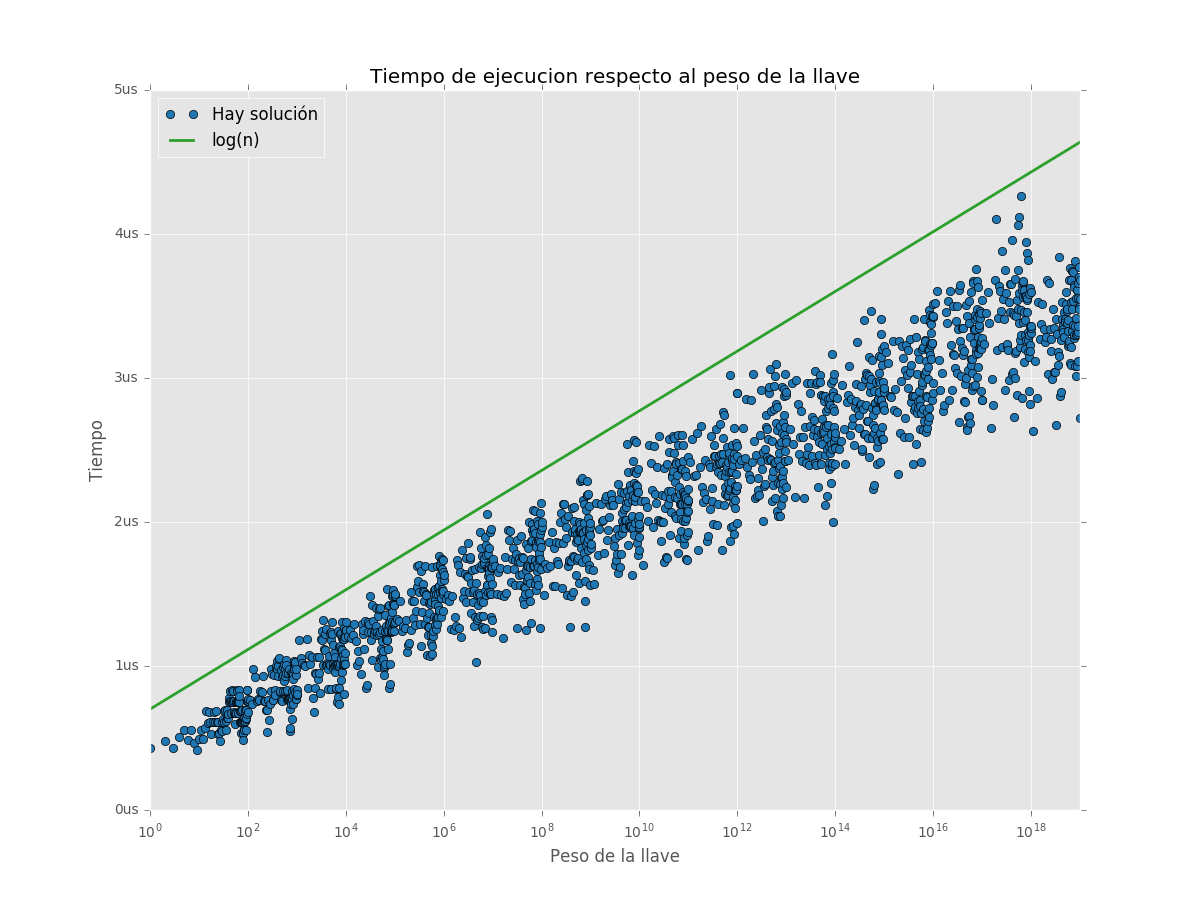
\includegraphics[width=\textwidth]{ej2-all}
    \caption{Tiempo de ejecución del algoritmo en función de P. Cada medición es el tiempo mínimo (considerando que toda distorsión entre las muestras empeora a lo sumo la performance pero nunca la mejora) de 10 corridas.}
    \label{fig:ej2-fig}
\end{figure}

	Los casos se generan con el criterio de distribuir, en los intervalos $[10^i$..$10^i+1]$ para $0 < i < 19$ (la cota superior se debe a la capacidad del tipo \emph{uint64_t} de \emph{C++}), un caso cada $10^{i-1}$ valores de $P$ \footnote{Para el intervalo de 0 a 10, son 10 mediciones para cada valor entero.}. La razón de esto es que en la sección anterior sugerimos una complejidad de orden logarítmico sobre el tamaño de la variable $P$ y una manera de contrastar empíricamente esto es notar un crecimiento lineal en el tiempo de ejecución para un eje de coordenadas exponencial para $P$, como podemos apreciar efectivamente en la figura \ref{fig:ej2-fig}.

	Otro punto de interés experimental, a raíz del control de flujo del código, es la \emph{'pinta'} que tiene la descomposición de $P$. Si bien el costo de peor caso de cada rama es constante, en algunos casos tendremos que realizar una mayor cantidad de operaciones, algunas de las cuales obligan siempre a realizar inserciones en alguno de los vectores. Además, en el caso de que el dígito actual sea nulo y no haya acarreo, no se ejecuta ninguna rama.

	\begin{figure}[H]
	    \centering
	    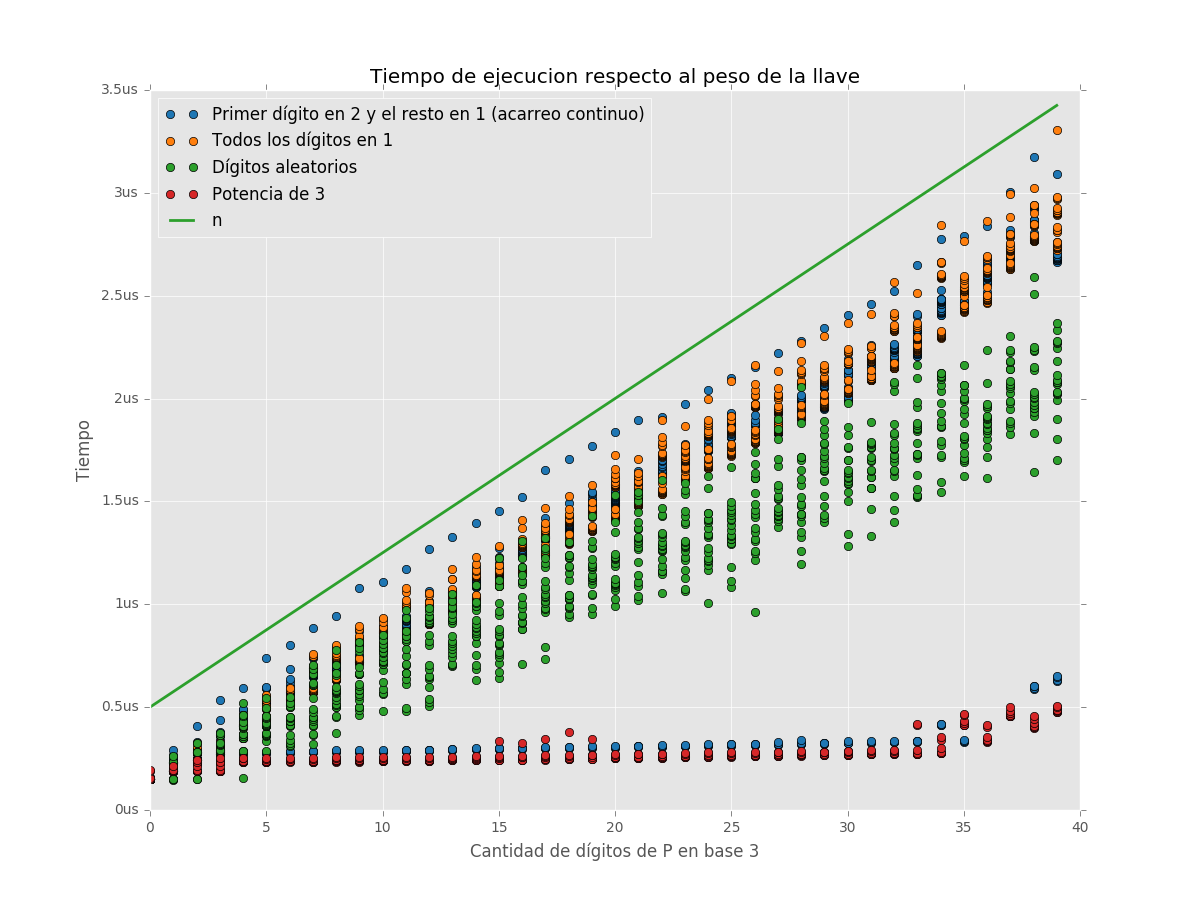
\includegraphics[width=\textwidth]{ej2-comp}
	    \caption{Tiempo de ejecución del algoritmo en función de la cantidad de dígitos de $A_3$ (como ya hablamos, de orden logarítmico en la variable $P$) para distintas características de su distribución. Nuevamente, cada medición es el tiempo mínimo de 10 corridas.}
	    \label{fig:ej2-comp}
	\end{figure}

	Cuando $P$ es una potencia de 3 no se entra en ninguna rama para ningún dígito que no sea el último, por lo tanto el tiempo de ejecución es el más bajo de todos. En los casos que armamos con el primer dígito de la representación siendo un 2 y el resto 1, de modo que la primer iteración produzca un acarreo que se va sosteniendo para cada uno de los dígitos siguientes teniendo que entrar en la rama del acarreo y además realizar inserciones en un vector, sucede algo extraño: en general el rendimiento es efectivamente peor que los casos aleatorios (que pueden contener ceros y entrar en menos ramas) como se esperaría, pero también existen casos en los cuales el rendimiento roza la optimalidad del caso potencia de 3. Sin embargo, considerando que siempre se entra exactamente en las mismas ramas durante toda la ejecución, es posible que exista una distorsión causada por el \emph{branch predictor}\footnote{https://en.wikipedia.org/wiki/Branch_predictor} del mismo procesador (lo cual también juega en favor del caso potencia, dado que va a tener tendencia a predecir que no se entre en ninguna rama). Curiosamente, el caso en que todos los dígitos son 1, que ejecuta de una manera similar al de los acarreros pero no entrando en el primer $if$, no parece afectado por el predictor.
